\chapter{Tecnologie utilizzate}
\label{ch:technologies}
Per lo sviluppo del progetto sono stati implementati diversi componenti sia lato hardware che software. 
In questo capitolo verranno riportate tutte le tecnologie adottate illustrandone una breve dscrizione.

\section{Raspberry}
\label{sec:raspberry}
Per la realizzazione della ``\texttt{cassetta delle lettere smart}'' (esposta nella Sezione ~\ref{sec:solution}) inizialmente si era pensato di utilizzare la piattaforma 
hardware Arduino \footnote{https://store.arduino.cc/arduino-uno-rev3}, successivamente si è optato però per la scheda Raspberry Pi in quanto quest'ultima più 
performante e meglio equipaggiata rispetto Arduino.

In particolare è stata utilizzata una scheda RaspberryPi 3 Model B \footnote{https://www.raspberrypi.org/products/raspberry-pi-3-model-b/} illustrata in 
Figura~\ref{photo_raspberry}.

Sviluppato dalla fondazione britannica no-profit Raspberry Pi Foundation il 29 Febbraio del 2012~\cite{stroyOFraspberry_Raspbian}, il progetto nacque per stimolare 
l'insegnamento dell'informatica e della programmazione nelle scuole e per promuovere lo studio del linguaggio di programmazione Python, da cui ne deriva la sigla 
Pi del logo.
Questa scheda fra l'altro ebbe successo anche grazie al bassissimo costo, infatti le prime due versioni costavano solo 25 e 35 dollari, rispettivamente 
per la versione da 256 e 512 Mb di RAM.
\begin{figure}[htb]
    \centering
    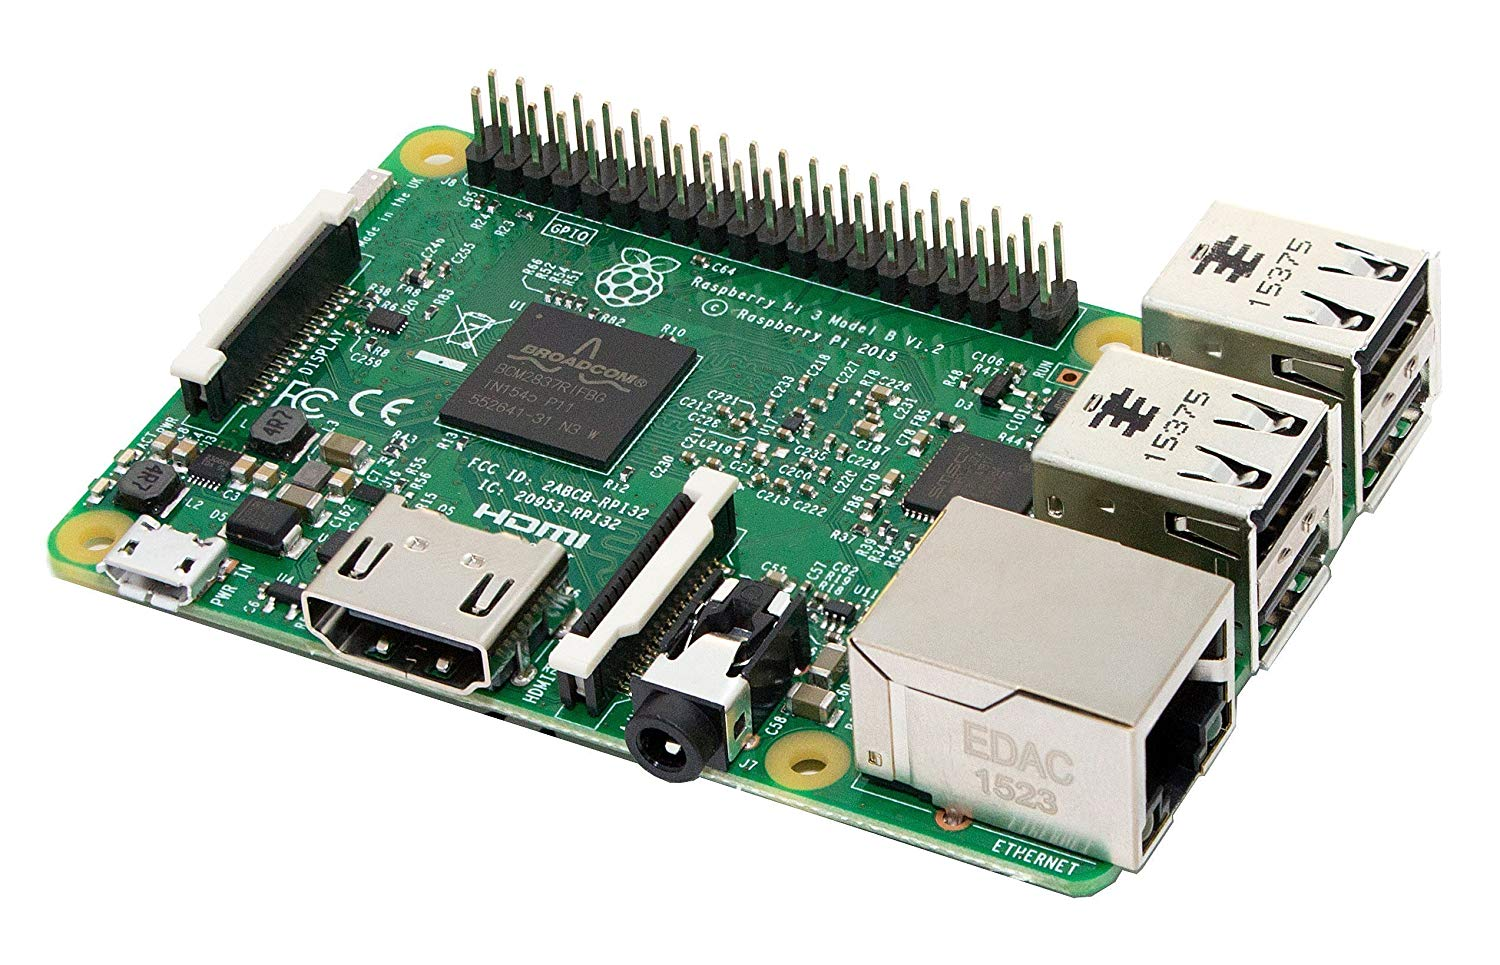
\includegraphics[width=0.7\textwidth]{images/raspberryPI.png}
    \caption{Raspberry Pi 3 Model B.}
    \label{photo_raspberry}
\end{figure}

Le specifiche tecniche della scheda Raspberry Pi 3 Model B sono:
\begin{itemize}
    \item Tensione di alimentazione: \textit{5V/2.5A DC}
    \item SoC: \textit{Broadcom BCM2837 Quad Core Cortex-A53 a 1.2 GHz, 32 kB L1 e 512 kB L2}
    \item GPU: \textit{Broadcom VideoCore IV Dual Core a 400 MHz}
    \item RAM: \textit{1GB LPDDR2 a 900 MHz}
    \item Rete: \textit{Ethernet 10/100, WiFi b/g/n 2.4 GHz, Bluetooth 4.1 con Bluetooth Low Energy(per un consumo di energia ridotto)}
    \item Porte: \textit{microSD, HDMI 1.4 CEC, jack 3.5 mm, 4 porte USB 2.0 (SMSC LAN9514)}
    \item Interfacce: \textit{CSI Camera Connector, DSI  Display Connector, GPIO header 40-pin}
    \item \textit{Slot per memoria microSD su cui viene installato il sistema operativo}
    \item Dimensioni: \textit{85 x 56 x 17 mm}
\end{itemize}

Le linee GPIO (General Purpose Input/Output), in FIgura~\ref{photo_gpio}
\footnote{www.element14.com/community/docs/DOC-73950/l/raspberry-pi-3-model-b-gpio-40-pin-block-pinout}, 
sono dei collegamenti tra il processore e i pin del 
connettore della scheda. Queste linee possono essere programmate per funzionare sia come porte di ingresso che come porte di uscita.

\begin{figure}[htb!]
    \centering
    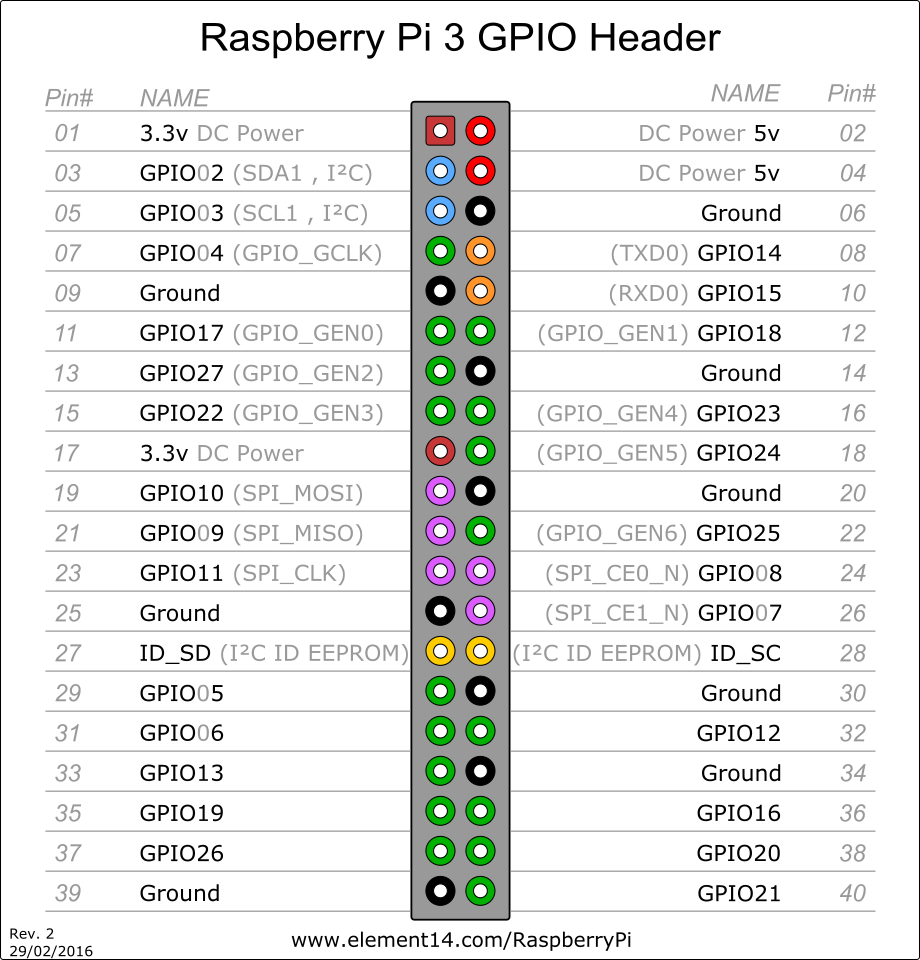
\includegraphics[width=0.7\textwidth]{images/gpio.png}
    \caption{Pin GPIO (General Purpose Input Output).}
    \label{photo_gpio}
\end{figure}

I 40 GPIO offerti dalla scheda Raspberry includono pin digitali, SPI, I2C e alimentazione 3V e 5V, esistono due differenti modalità per indicare uno specifico pin , il 
sistema BOARD ed il sistema BCM.

Il sistema BOARD fa riferimento alla loro posizione fisica, quindi effettivamente, il pin 1 risulterà essere 3.3V PWR, mentre ad esempio, riferendoci al pin 16 interagiremo 
con il pin GPIO23 (GPIO\textunderscore GEN4).

Il sistema BCM, invece,  si riferisce ai pin GPIO che sono stati direttamente collegati al SoC(``cervello'' del Pi) della scheda ed avrà quindi un modo 
differente per chiamare lo stesso pin. Ad esempio, il pin in posizione 16 visto prima, sarà chiamato GPIO23.

Per usare questi pin con questi protocolli, sono state importate una delle tante librerie Python disponibili, infine, sono state abilitate le interfacce usando l’applicazione 
Raspberry Pi Configuration disponibile nel sistema operativo Raspbian, nel menu Preferenze.


\subsection{Rasbian}
Per la scheda Raspberry è stato installato il sisitema operativo ufficiale Rasbian, identificato dall'immagine in Figura~\ref{photo_raspbian}, una 
distribuzione di Linux Debian costruita appositamente per il Raspberry Pi, il nome nasce dalla contrazione dei termini Raspberry Pi e Debian, sviluppato da 
Mike Thompson e Peter Green nel Giungno del 2012~\cite{stroyOFraspberry_Raspbian} con una build iniziale di oltre 35.000 pacchetti precompilati di software in bundle
in un formato adatto per una semplice installazione sulla scheda.

Rispetto Debian, Raspbian alleggerisce notevolmente il carico della CPU nell'esecuzione del sistema grazie a importanti modifiche dell'interfaccia grafica, questo 
anche date le limitate prestazioni della scheda. 
\begin{figure}[htb]
    \centering
    
\includegraphics[width=0.7\textwidth]{images/raspbian.png}
    \caption{Logo Raspbian.}
    \label{photo_raspbian}
\end{figure}

Per quanto riguarda le funzionalità offerte, questo è un sistema operativo discretamente completo, infatti grazie a un costante sviluppo la quantità dei software 
presenti è continuata a crescere arrivando a contenere persino programmi di elaborazione di testi o client di posta elettronica.


\subsection{Raspberry Pi Camera}
La fotocamera utilizzata per scattare le foto del mittente è la Raspberry Pi camera Module V2, in Figura~\ref{photo_camera}, un prodotto ufficiale della Raspberry Pi 
Foundation, il modello originale da 5 megapixel è stato rilasciato nel 2013 mentre quello utilizzato nel progetto è stato rilasciato nell'Aprile del 2016.

Dotata di un sensore di alta qualità da 8 megapixel Sony IMX219 appositamente disegnato con obiettivo a fuoco fisso è in grado di scattare foto da 3280x2464 pixel e 
supporta video da 1080p30, 720p60 e 640x480p60/90, si installa sulla scheda Raspberry tramite l'interfaccia CSi appositamente dedicata tramite il cavo flessibile in 
dotazione, è molto comoda e poco ingombrante grazie al ridotto peso di 3g con una grandezza pari a 25mm x 23mm x 9mm.
\begin{figure}[htb]
    \centering
    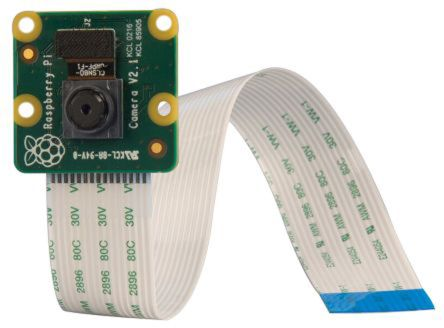
\includegraphics[width=0.7\textwidth]{images/piCamera.png}
    \caption{Raspberry Pi camera Module V2.}
    \label{photo_camera}
\end{figure}


\subsection{Qwiic Proximity Sensor (VCNL4040)}

Come illustrato nella sezione~\ref{sec:solution}, l'utente viene avvisato della ricezione di nuova posta ogni volta in cui viene introdotta una lettera nel bucalettere,
per rilevarne il passaggio è stato utilizzato il sensore Qwiic Proximity Sensor (VCNL4040), in Figura~\ref{photo_sensor}, un semplice sensore a infrarossi in grado di 
rilevare il passaggio di oggetti fino ad una distanza di circa 20cm.
\begin{figure}[htb]
    \centering
    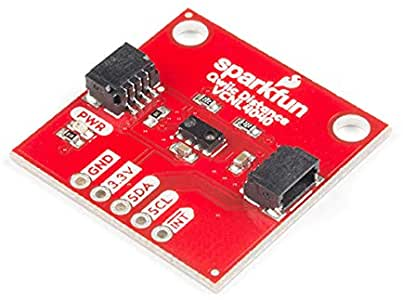
\includegraphics[width=0.7\textwidth]{images/sensor.png}
    \caption{Sensore di prossimità a infrarossi Qwiic VCNL4040.}
    \label{photo_sensor}
\end{figure}

Il sensore non ha punti morti, è in grado quindi di rilevare il passaggio di oggetti vicinissimi non determinandone una distanza esatta ma indicando se l'oggetto è più 
vicino o lontano rispetto l'ultima lettura effettuata, problema che non sussiste dal momento che sarà sufficente rilevare solo il passaggio 
della lettere senza specificare a quale distanza sia passata.



\section{Python}
\label{sec:python}
Il linguaggio di programmazione utilizzato per la realizzazione di questo progetto è Python, in particolare la versione 3.6.

Nel 1991 Guido Van Rossum, avute alcune idee mirate al miglioramento di ABC~\footnote{https://it.wikipedia.org/wiki/ABC\_(linguaggio)}, si mise a lavorare allo 
sviluppo di un nuovo linguaggio di programmazione, nasce così Python, la scelta del nome venne influenzata dalla passione dello sviluppatore per il gruppo comico 
inglese Monty Python.

Python è un linguaggio multi-paradigma che riesce a sfruttare il paradigma object oriented, la programmazione strutturata così come la  programmazione funzionale, le 
variabili sono non tipizzate e viene usata l'indentazione per definire il corpo di metodi, cicli, classi ecc\dots

Il controllo dei tipi viene eseguito a runtime ed è di tipo forte (strong typing~\footnote{https://it.wikipedia.org/wiki/Tipizzazione\_forte}), le variabili in questo 
linguaggio sono paragonabili a dei contenitori ai quali viene associato un nome, il quale consente di riferirsi in ogni momento alla variabile(contenitore) associata, 
ogni contenitore è associabile a diversi altri contenitori anche di altro tipo(String, Int, Double, ecc\dots) durante il suo tempo di vita, cioè fino a quando il 
garbage collector procede alla liberazione automatica della memoria non appena si verificano le opportune condizioni.

Python è oggi uno dei linguaggi più utilizzati in assoluto per l'estrema capacità di adattamento a tutte le esigenze e quindi applicabile in svariati ambiti, ad
esempio lo si può utilizzare per la programmazione di interfaccie grafiche(GUI) o sviluppo Web.
Nel corso del tempo si è assistito ad una vera e propria evoluzione del linguaggio, questo soprattutto dovuto al fatto d'essere open source e quindi tutti hanno 
contribuito a migliorarlo, la sua diffusione è dovuta anche a diversi vantaggi offerti, tra i tanti infatti Pyton:
\begin{itemize}
    \item È facile da usare in quanto la sintassi e i diversi moduli e funzioni che sono già inclusi nel linguaggio sono consistenti, intuitivi, e facili da imparare.
    \item È ricco di librerie con una collezione di oltre 200 moduli per svolgere i compiti più disparati.
    \item È performante, i programmi infatti vengono automaticamente compilati in un formato chiamato bytecode (formato più compatto ed efficiente, 
    garantisce quindi prestazione elevate) prima di essere eseguiti.
    \item È portabile, viene utilizzato su svariate piattaforme come : Windows, Linux, Unix, Macintosh e su cellulari Android e iOS, lo stesso codice quindi può essere 
    eseguito su qualsiasi piattaforma purché abbia l'interprete Python installato.
\end{itemize}



\section{Librerie utilizzate}
\label{sec:library}
Come fatto presente nella sezione~\ref{sec:python} è stato utilizzato Python come linguaggio di programmazione, sono state utilizzate varie librerie riportate in 
dettaglio nelle sezioni a seguire per vari scopi fra cui:
\begin{itemize}
    \item Interagire con il sensore e la fotocamera collegati alla scheda Raspberry Pi 3 Model B.
    \item Avere accesso ai servizi offerti da AWS.
    \item Utilizzare i server e-mail per inviare e ricevere e-mail.
    \item Far scattare un contatore che tiene conto del tempo trascorso e quindi eseguire delle operazioni preimpostate.
\end{itemize}


\subsection{Boto3}
\label{sec:boto3}
Boto è il Software Development Kit (SDK) di Amazon Web Services (AWS) per Python, che consente agli sviluppatori Python di scrivere software che utilizza servizi 
come Amazon S3 e Amazon EC2, per utilizzarlo come consultabile nell'appostia guida~\cite{boto3}, è stato insatallato in locale(sulla scheda Raspberry) con il comando
\textbf{pip install boto3 } e succesivamente configurato opportunamente.

Boto3 è un'applicazione che fornisce supporto nativo in Python, offre un'API orientata agli oggetti facile da usare e un accesso diretto al 
servizio di basso livello, vengono messi a disposizione due livelli di API: 
\begin{enumerate}
    \item Le API client (o di "basso livello") che forniscono mappature univoche alle operazioni API HTTP.
    \item Le API di risorse (o di "alto livello") che eseguono chiamate di rete esplicite, fornendo oggetti e raccolte di risorse per accedere agli attributi 
    ed eseguire azioni.
\end{enumerate}
Numerose richieste che utilizzano boto3 non sono istantanee, in alcuni casi questo non è un prblema, infatti è possibile fare una richiesta e controllare in un secondo
momento se è stata completata o meno, in altri casi invece, desideriamo attendere il completamento della richiesta prima di passare alle parti successive dello 
script che potrebbe fare affidamento ad un processo più lungo per essere completato, in questi casi è possiblie utilizzare dei ``waiter'' inclusi in Boto3, 
i quali ricercano in modo continuo eventuali modifiche agli stati predefiniti nelle risorse AWS, un esempio potrebbe essere quello di uno script che copia un AMI
(Amazon Machine Image)~\footnote{https://docs.aws.amazon.com/it\_it/AWSEC2/latest/UserGuide/AMIs.html}
su un altro account condividendo tutte le istantanee. Dopo aver condiviso le istantanee con l'altro account, è necessario attendere il completamento delle copie 
dell'istantanea locale prima di registrare l'AMI nell'account di ricezione.


\subsection{E-mail}

E-mail è una libreria che permette la gestione di messaggi di posta elettronica, inclusi MIME e gli altri documenti basati sulla RFC 2822, divide l'analisi e la 
generazione del messaggio di e-mail dal modello oggetto di rappresentazione interno dell'e-mail. 
Il package e-mail non è specificamente progettato per nessun invio di messaggi di posta tramite server SMTP (RFC 2821), questa è la funzione del modulo smtplib 
utilizzato in questo progetto come vedremo più avanti.

Il componente centrale del pacchetto è un "modello a oggetti" che rappresenta i messaggi di posta elettronica, un'applicazione interagisce con il pacchetto 
principalmente attraverso l'interfaccia del modello a oggetti definita nel sottomodulo dei messaggi eseguendo diverse operazioni come ad esempio rimuovere gli 
oggetti secondari dai messaggi, riorganizzare completamente il contenuto, etc\dots

Ci sono altri due componenti fondamentali del package e-mail e sono, l'analizzatore (il parser) e il generatore.
Il parser accetta in input la versione serializzata di un messaggio di posta elettronica (uno stream di bytes) e li converte in un albero di oggetti EmailMessage,
il generatore prende un EmailMessage e lo trasforma in un flusso di byte serializzato, sono presenti anche utili sotto classi per alcuni tipi di oggetti MIME comuni, 
ed alcune utilità generiche che aiutano con alcuni compiti comuni.

In questo progetto, è stato necessario avere la possibilità di inviare e 
ricevere posta elettronica, per far ciò sono state usate due librerie, smtlib\footnote{https://docs.python.org/3/library/smtplib.html} per l'invio di posta elettronica
mentre imaplib\footnote{https://docs.python.org/2/library/imaplib.html} per la ricezione.

\subsection{Picamera}
Questo pacchetto fornisce un'interfaccia Python per la videocamera Raspberry Pi, è disponibile in diverse verisoni, Python 2.7 (o versioni successive) 
o Python 3.2 (o versioni successive), il codice è concesso in licenza da BSD license~\footnote{https://opensource.org/licenses/BSD-3-Clause}.

Utilizzando questa libreria è possibile scrivere dei programmi che ci permettono di scattare immagini, girare filmati per poi elaborarli successivamente, 
inoltre grazie ai pin GPIO è possibile integrare l’uso della telecamera con sensori o interruttori.

\subsection{Adafruit vcnl4040}

Questa è la libreria di sensori di prossimità e luce ambientale Adafruit VCNL4040, sviluppata da Kattni Rembor, è stata testata e funziona perfettamente con 
il sensore adottato.

Il chip scelto ha bisogno di 2 pin per interfacciare Adafruit e utilizza il protocollo I2C per comunicare, creato da Philips, 
questo protocollo di comunicazione seriale sincrono, permette a diversi dispositivi lo scambio di dati utilizzando solo due fili collegati negli appositi pin GPIO,
in FIgura~\ref{photo_gpio}, uno viene utilizzato per l'invio dei dati mentre l'altro per sincronizzare la comunicazione.
 
\subsection{Time}

La libreria Time offre varie funzioni della libreria in linguaggio C per la maipolazione di date e tempo, visto che è legato all'implementazione in C, 
alcuni dettagli (come l'inizio dell'epoca ed il valore massimo di data supportato) sono specifiche alla piattaforma.

L'istante da cui inizia il conteggio del tempo e dato da ``epoch'', le funzioni in questo modulo non gestiscono i tempi e le date prima di ``epoch'' o molto lontane 
nel futuro, per i sistemi Unix epoch è il 1970, per cui ad esempio il primo gennaio di quell'anno, all'ora 0, il tempo trascorso da epoch è 0, mentre il punto di 
interruzione nel futuro, sempre nei sistemi Unix, è di solito l'anno 2038.


\section{Amazon Web Services}
\label{sec:aws}
Amazon Web Services (o AWS), azienda statunitense di proprietà del gruppo Amazon, è una piattaforma che offre servizi in cloud computing, rivolta a tutte quelle
imprese o Pubbliche Amministrazioni che intendono innovare e potenziare il loro reparto IT e la loro strumentazione informatica, è possibile trovare tra i più
disparati servizi come database, realtà aumentata e virtuale, Internet of Things, calcolo, servizi multimediali e molto altro ancora.

AWS si sta affermando rapidamente ovunque nel mondo, questo perchè ogni servizio proposto è altamente scalabile, veloce ed affidabile e per i numerosissimi 
servizi offerti che a oggi sono oltre 150, nonostante ciò il Provider non smette di popolarlo aggiungendo quasi ogni mese nuovi prodotti.

Contrariamente a quanto si pensa, le fonti di guadagno del gruppo Amazon provengono proprio da AWS, come è possibile constatare dai dati pubblicati nel 
quarto trimestre del 2018~\cite{aws}, AWS rappresenta per Amazon il 58\% dei guadagni totali, rendendola così la sua più grande fonte di incassi.
Nelle sezioni a seguire verrano illustrati nel dettagio i servizi utilizzati. 

\subsection{Amazon Simple Storage Service}
Amazon Simple Storage Service (Amazon S3) è un servizio che permette di memorizzare grandi quantità di dati. Il servizio può essere gestito tramite console AWS o con
Amazon s3 API, tra i vantaggi offerti ci sono:
\begin{itemize}
    \item Affidabilità: progettato per una durabilità del 99,999999999\% e per la memorizzazione di dati.
    \item Storage illimitato: nessun limite alla quantità di dati archiviabili.
    \item Sicurezza: gestione meccanismo di autenticazione.
    \item Scalabilità: spazio disco, numero di richieste e utenti. Non si deve pensare alla necessità di spazio futuro. 
\end{itemize}
Amazon S3 è composto da bucket indentificati da un nome univoco a livello modiale, per ogni regione, questo perché deve essere raggiungibile via web da una url univoca,
bisogna scegliere una regione specifica per un'esigenza di tipo normativo e ottimizzazione della latenza.

Un bucket è un contenitore di oggetti memorizzati in Amazon S3, ogni oggetto all'interno del bucket è identificato univocamente da una chiave (key), gli oggetti sono 
composti dal dato vero e proprio(foto, testo ecc\dots) ed eventualmente i metadata, che sono una coppia nome-valore che descrivono l'oggetto.

\subsection{Amazon DynamoDB}
Amazon DynamoDB è un servizio di database non relazionale per qualsiasi scala, combina prestazioni elevate e prevedibili con una scalabilità ottimale, è possibile 
creare tabelle di database in grado di archiviare e recuperare qualunque quantità di dati e soddisfare qualsiasi livello di traffico richiesto.

DynamoDB memorizza i dati in tabelle, una tabella è una raccolta di dati che contiene zero o più item, quando viene creata, oltre al nome della tabella bisogna 
specificare anche la chiave primaria della tabella, il cui compito è quello di identificare univocamente ciascun item della tabella, in modo da evitare la ripetizione
della stessa chiave su item diversi. 

Un item è un set di attributi identificabili in modo univoco tra tutti gli altri item, in questo database non relazionale gli elementi sono simili per molti aspetti 
alle righe, ai record o alle tuple in altri sistemi di database.

In DynamoDB, è possibile memorizzare un numero arbitrario di item in una tabella, ogni item è composto da uno o più attributi. Un attributo è un elemento dati 
fondamentale che non ha bisogno di essere ulteriormente suddiviso, gli attributi sono simili per molti aspetti ai campi o alle colonne presenti in altri sistemi 
di database.

\subsection{AWS Lambda}
AWS Lambda è un servizio di elaborazione senza server (serverless) che esegue un determianto codice, scritto dalla console o caricato come vedremo più avanti, in 
risposta a determinati eventi, che possono essere ad esempio modifiche agli oggetti (inserimento, modifica, eliminazione) in un bucket Amazon S3, l’aggiornamento di 
tabelle in Amazon DynamoDB, ecc\dots

Uno dei tanti pregi di AWS Lambda sono i prezzi contenuti, infatti la tariffa è calcolata su intervalli di 100 millisecondi di esecuzione del codice e per il numero di 
volte in cui viene attivato, quindi in poche parole i prezzi sono calcolati in base al tempo effettivo di elaborazione. 

Il codice che si decide di eseguire su AWS Lambda prende il nome di ``funzione Lambda", una volta creata, una funzione Lambda è sempre attiva e pronta per essere 
lanciata. Alla creazione della funzione quindi, bisogna attribuirle un nome, caricare il codice da locale oppure creandola direttamente dalla console di 
Lambda, scegliere la memoria utilizzata, il periodo di timeout e il ruolo AWS Identity and Access Management (IAM), a questo punto bisogna solo specificare quando 
lanciare la funzione, come abbiamo visto in precedenza, questo è possbilie in risposta a degli eventi, così al variare della risorsa, Lambda eseguirà la funzione e 
avvierà e gestirà le risorse di elaborazione necessarie in base alle richieste in entrata, inoltre dal momento che le funzioni Lambda sono "stateless", cioé prive di 
affinità con l'infrastruttura sottostante, potranno essere avviate un numero qualsiasi di copie della funzione, in base alla frequenza degli eventi in entrata.

\subsection{Amazon Rekognition}
Amazon Rekognition è il servizio AWS che nel progetto realizzato riconosce il volto del mittente, possibile grazie all'utilizzo di una tecnologia di deep learning 
sicura e altamente scalabile il cui utilizzo non richiede competenze di machine learning.

Questo servizio è in grado di identificare automaticamente e in tempo reale, alcuni attributi e comprendere ad esempio se una faccia è felice o meno o se due facce con 
espressioni differenti sono associate alla stessa persona, tutto ciò analizzando immagini o video sia archiviati in precedenza che in streaming.

La risorsa principiale di Amazon Rekognition è la raccolta dei volti (collection), un ``container" lato server contenente una serie di informazioni, 
per ogni volto infatti, viene utilizzata l'analisi facciale per estrarre informazioni multidimensionali sulle caratteristiche facciali, quindi viene calcolato un
ID alfanumerico che identifica univocamente il volto corrispondente(FaceId), per far ciò è stata usata come vedremo nel capitolo ~\ref{ch:development} la funzione 
IndexFaces.

Il riconoscimento di un volto è suddiviso in 2 fasi fondamentali:
\begin{itemize}
    \item \textbf{Indicizzazione dei volti:} al volto in input viene associato un ID che identifica univocamente il volto correntemente analizzato, non 
    è possibile accedere direttamente a queste informazioni tuttavia, Amazon Rekognition utilizza queste informazioni quando viene cercata una corrispondenze di volti.
    \item \textbf{Ricerca dei volti:} in questa fase si procederà analizzando il volto in input e confrontandolo a uno dei volti presenti nella raccolta dei volti 
    utilizzando l'algoritmo di Amazon Rekognition.
\end{itemize}

\subsection{Amazon CloudWatch}

Amazon CloudWatch è un servizio web che permette la monitorazione ed il controllo delle risorse utilizzate da molti servizi AWS, il che è utile per la 
comprensione di problemi di performance e/o le risorse necessarie al funzionamento delle applicazioni utilizzate. 

Con questo servizio è possibile monitorare le prestazioni operative, l’utilizzo delle risorse, il traffico di rete, impostare allarmi che tramite il servizio Amazon 
SNS possono generare diversi messaggi, visualizzare grafici e ottenere statistiche per i dati metrici.
Ad esempio è possibile controllare il risultato dell'esecuzione della funzione Lambda,il livello di CPU utilizzato dalle istanze EC2, la quantità del trasferimento 
dati, ecc\dots

Per l'utilizzo di questo servizio è suffciente accedere alla management console e selezionare il menu dedicato al servizio, a questo punto si viene reindirizzati in una
pagina in cui si trovano due sezioni, una per le metriche e l’altra per gli allarmi. 
Nella sezione dedicata alle metriche sono presenti tutte le statistiche raccolte riguardanti i servizi utilizzati, in quella dedicata agli allarmi 
invece è possibile impostare delle soglie il cui superamento innesca l'emissione di apposite notifiche.
Nel progettato realizzato questo servizio è stato utilizzato per testare e verificare il corretto funzionamento della funzione AWS Lambda.


\subsection{AWS Identity and Access Management}
\label{sec:iam}
Le teconologie sviluppate ai giorni nostri stanno rendendo sempre meno efficaci e obsoleti tutti i parametri di sciurezza utilizzati per la difesa del 
perimetro fiscio aziendale. 

Per difendersi efficacemente da attacchi sempre più efficaci e pericolosi bisogna adeguarsi di conseguenza, infatti adesso per la 
sicurezza informatica il principio fondamentale non è più il ``dove'' si trovano le risorse ma ``chi'' ne ha accesso, ed è qui che entra in gioco il servizio AWS 
Identity and Access Management (o brevemente ``IAM"), i sistemi IAM sono in grado di impedire agli hacker l'accesso alle applicazioni, ai privilegi e ai dati sensibili
quando vengono compromesse le credenizli di un dipendente.

È possibile interagire con IAM tramite AWS Command Line Interface(AWS CLI), la console IAM, l'API AWS o gli SDK di AWS. Questo servizio offre la possibilità di creare 
identità IAM (come utenti, gruppi, ruoli) e assegnare set di autorizzazioni personalizzate (policy IAM) a tali identità, le policy possono essere predefinite o create 
dall'utente, vengono utilizzate in quanto consentono ai clienti di controllare dettagliatamente chi è in grado di accedere a una risorsa specifica e come può usarla 
all'interno di tutto l'ambiente cloud.


\section{GitLab}
\label{sec:git}
Si è scelto di usare un servizio di hosting di codice come GitLab per la gestione delle varie verisoni o modifiche del codice, questo anche per rendere più agevole 
l'aiuto da parte del professore su problematiche software o hardware.

GitLab è una piattaforma web open source appartenente a GitLab Inc, di base l'interazione è possibile tramite linea di comando per cui per agevolarne l'utilizzo si 
può ricorrere a un’interfaccia grafica che ne semplifichi l’utilizzo.
In Git ci sono quattro concetti base che sono:
\begin{enumerate}
    \item \textbf{Snapshot(istantanee):} permettono di tenere traccia della cronologia del codice registrando lo stato attuale di tutti i file in un dato momento. 
    Utile agli utenti in quanto deciso su quale file creare uno snapshot, permette di effettuare il rollback o identificare modifiche e bug.
    \item \textbf{Commit:} è l’azione con la quale si genera uno snapshot, in altre parole i commit rappresentano il modo in cui si ``salvano” le modifiche fatte al 
    codice. Nello specifico il commit corrisponde al salvataggio di uno o più file aggiornati sul repository.
    \item \textbf{Repository:} è una collezione di tutti i file del progetto che comprendono anche la cronologia e storico dei commit. Possono essere eseguite 4 azioni al 
    repository:
    \begin{itemize}
        \item Init: inizializza un nuovo repository all’interno della cartella corrente.
        \item Clone: clona un repository Git esistente dal server remoto.
        \item Pull: scarica dati da un repository remoto.
        \item Push: invia branch e dati a un repository remoto.
    \end{itemize}
    \item \textbf{Branch:} Git archivia i file e li tiene ordinati in una struttura ad albero, il branch è una diramazione di tale struttura. Tutti i commit risiedono 
    su qualche branch, quello primario per impostazione predefinita si chiama master ed è possibile avere branch multipli in un singolo repository.
\end{enumerate}